% Created 2020-04-08 Wed 12:18
% Intended LaTeX compiler: pdflatex
\documentclass[11pt]{article}
\usepackage[utf8x]{inputenc}
\usepackage[T1]{fontenc}
\usepackage{graphicx}
\usepackage{grffile}
\usepackage{longtable}
\usepackage{wrapfig}
\usepackage{rotating}
\usepackage[normalem]{ulem}
\usepackage{amsmath}
\usepackage{textcomp}
\usepackage{amssymb}
\usepackage{capt-of}
\usepackage{hyperref}
\usepackage{unicode-math}
\author{Gianluca Scarpellini (gianluca@scarpellini.dev)}
\date{\today}
\title{Project 2 - Deep reinforcement learning - Continuous Control}
\hypersetup{
 pdfauthor={Gianluca Scarpellini (gianluca@scarpellini.dev)},
 pdftitle={Project 2 - Deep reinforcement learning - Continuous Control},
 pdfkeywords={},
 pdfsubject={},
 pdfcreator={Emacs 26.3 (Org mode 9.3.6)}, 
 pdflang={English}}
\begin{document}

\maketitle
\tableofcontents


\section{Introduction}
\label{sec:org8397757}
Deep Reinforcement Learning is today becoming a relevant field of research. The
current work aims to evaluate the ability of value-based methods of solving a
simple task in a constrained environment. In particular, we implemented Deep
DPG algorithm as presented during Udacity "Deep Reinforcement Learning"
as well as in the original paper. We describe the environment in section
\ref{sec:org754b3bc}. A more in depth explanation of the approach is presented in
section \ref{sec:org1fc6b2c}. In section \ref{sec:orgc49d0de} we comment the results
obtained with the algorithm. Finally, we take our conclusions in section
\ref{sec:org8dd118b}. 


\section{Environment and task}
\label{sec:org754b3bc}
The presented project is developed in order to solve the "Reacher" environment
with multiple agents (20 agents were employed for this specific project). The
tasks consists in moving a double-jointed arm to target locations. The reward is
+0.1 for each correct movement. The agent goals is to maintain the right
position as along as possible. The observation space consists of 33 values
(position, rotation, velocity, angular velocities for each arm). The space
action is \textbf{continuous}; each action is contained between -1 and +1.

\section{Algorithm and Implementation}
\label{sec:org1fc6b2c}
\begin{figure}[htbp]
\centering

\includegraphics[width=.9\linewidth]{../contents/actor_critic.png}
\caption{\label{fig:org8e45ddd}Actor-critic approach}
\end{figure}

We used an actor-critic approach to solve the environment. Actor-critic methods
merges the idea of \textbf{policy-based} and \textbf{temporal-differences} in order to
mitigate their issues both in variance and bias. DDPG exploits 2 different
function approximators (such as neural networks, CNN, \ldots{}). The policy produces
by the actor is \textbf{deterministic}: the action per state is the optimal one. The
critic evaluates the deterministic policy and updates its parameters using
TD-error. The \textbf{deterministic policy gradient algorithm} is employed to update
the actor weights following equation in figure \ref{fig:org9e577f9}.


\begin{figure}[htbp]
\centering
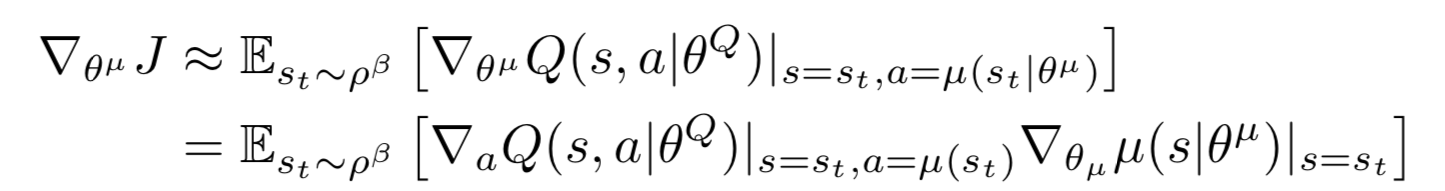
\includegraphics[width=.9\linewidth]{../contents/dpg.png}
\caption{\label{fig:org9e577f9}DPG equation}
\end{figure}

\subsection{Improvements}
\label{sec:org7537283}
We employed a few improvements proposed in the original DDPG article in order to
stabilize training.

\begin{itemize}
\item \textbf{Experience Replay}: The experience replay was originally proposed for Deep
Q-learning approach. It employs a buffer of finite size in order to sample
randomly from the state-action-rewards tuple space. Independent mini-batches
favor a more stable training.
\item \textbf{Soft updates}: In DDPG the target networks are updated using a \textbf{soft copy} of
the old weights. The result is a more smooth updating of neural networks
parameters.
\item \textbf{Parallelism}: We adapt DDPG in order to exploit a multi-agent
environment. The behavior of the algorithm is the same; the experience buffer
and the updates benefit from the high independence of the experiences coming
from different parallel agent.
\end{itemize}

\subsection{Hyperparameters}
\label{sec:orgcacea13}
For the experiment we used the following hyperparameters:

\begin{center}
\begin{tabular}{lr}
Hyperparameter & Value\\
\hline
Replay buffer size & 1e6\\
Batch size & 1024\\
\(\gamma\) & 0.99\\
\(\tau\) & 1e-3\\
Actor lr & 1e-4\\
Critic lr & 3e-4\\
Update every & 20\\
Update times & 10\\
Episodes & 500\\
\hline
\end{tabular}
\end{center}


\section{Results}
\label{sec:orgc49d0de}
In figure \ref{fig:org94af033} it's presented the algorithm result per episode. In
particular, we were able to solve the environment in less then 50 epochs. The
scores kept growing until an optimal maximum of 35, probably due to limited time
play per episode. The learning has been stable until 350 when it starts reaching
a local minimal. Different approaches and improvements are discussed in section \ref{sec:org8dd118b}. 

\begin{figure}[htbp]
\centering
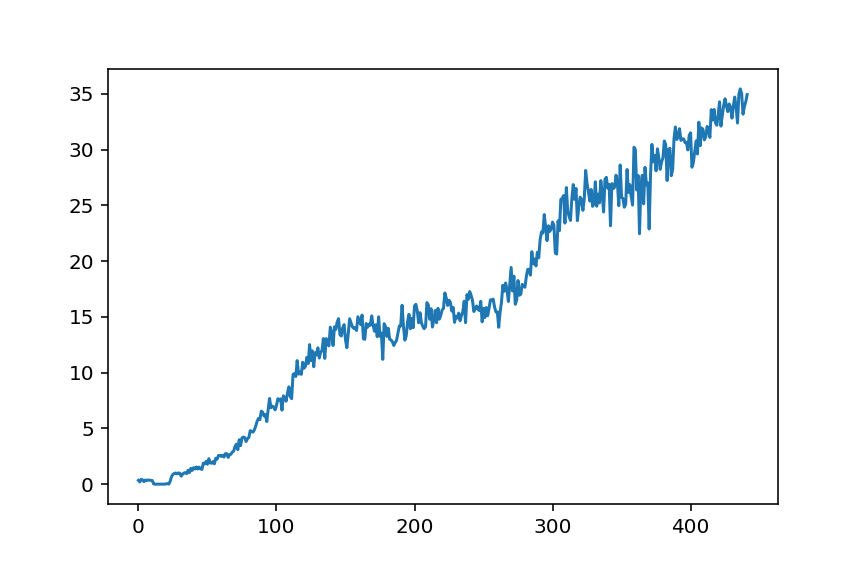
\includegraphics[width=.9\linewidth]{../contents/solved.png}
\caption{\label{fig:org94af033}Learning scores per epoch}
\end{figure}

\section{Conclusion and further}
\label{sec:org8dd118b}
We developed a pipeline in order to solve `reacher` environment with Deep
Reinforcement Learning. In particular, we implemented \textbf{Deep Deterministic Policy
Gradient} following the paper specification. DDPG is an off-policy actor-critic
algorithm which has proven stability and optimal results in multiple tasks. We
got the algorithm to hack the environment in less then 500 epochs. We believe
better results in terms of training speed could be achievable using more
advances algorithms like PPO for continuous action. As a matter of fact, PPO
could better benefit from the parallelism offered by the environment. We would
consider integrating \textbf{Prioritized Replay} as a way to optimally sample
mini-batches from the queue. 
\end{document}